\documentclass[12pt]{article}
\usepackage[a4paper, margin=1.5cm]{geometry}

\usepackage{xfp} % in preamble
\usepackage{graphicx}



\usepackage{customPackages/mylinks}
\usepackage{customPackages/loh_skills}
\usepackage{customPackages/loh_perks}

\usepackage{hyperref} % For links and references
\usepackage{makeidx}  % for the Indexing.

\usepackage{longtable}      % for the table itself
\usepackage{array}          % for \newcolumntype (centered text in table)

\usepackage{xparse}     % Optional Argument Stuff IfNoValueTF

\usepackage{graphicx}
\usepackage{multicol}
\usepackage{ragged2e}
\usepackage{lipsum}
\usepackage{fancyhdr}
\usepackage{makeidx}
\usepackage{hyperref}
\usepackage{parskip}
\usepackage{titlesec}
\usepackage{tikz}
\usepackage{eso-pic}
\usepackage{xcolor}
\usepackage{tabularx}
\usepackage{tabularray}
\UseTblrLibrary{booktabs}
\usepackage{longtable}
\usepackage{tocloft}
\usepackage{xcolor}
\usepackage{titlesec}

% used to get the full screen background image stuff to work
\newcommand\SetBackgroundImage[1]{%
  \AddToShipoutPictureBG*{%
    \put(0,0){%
      \parbox[b][\paperheight]{\paperwidth}{%
        \vfill
        \centering
        \includegraphics[width=\paperwidth,height=\paperheight]{#1}%
        \vfill
      }%
    }%
  }%
}

% used to get the full screen background image stuff to work
\newcommand\ClearBackgroundImage{%
  \ClearShipoutPictureBG
}

% Define a custom command for subsubsubsection
% these are NOT sections, but should allow us to play with headings and suchlike.
\usepackage{xcolor} % optional, for color
\newcommand{\subsubsubsection}[1]{%
  \vspace{1em} % vertical space before
  \noindent\textbf{\small #1}\par
  \vspace{0.5em} % vertical space after
}

\setcounter{secnumdepth}{-1} % Disable numbering for all section levels
\setcounter{tocdepth}{3}     % Show sections, subsections, subsubsections in TOC

% Remove numbers from TOC entries:
\usepackage{tocloft}
\renewcommand{\cftsecaftersnum}{}       % Remove section numbers in TOC
\renewcommand{\cftsubsecaftersnum}{}    % Remove subsection numbers in TOC
\renewcommand{\cftsubsubsecaftersnum}{} % Remove subsubsection numbers in TOC

% Adjust indentation for TOC entries
\setlength{\cftsecindent}{0pt}          % Section indent (usually zero)
\setlength{\cftsubsecindent}{0.5em}     % Subsection indent
\setlength{\cftsubsubsecindent}{1em}    % Subsubsection indent

% Optionally adjust the width reserved for numbers (to zero, since no numbers)
\setlength{\cftsecnumwidth}{0pt}
\setlength{\cftsubsecnumwidth}{0pt}
\setlength{\cftsubsubsecnumwidth}{0pt}

% "Style" Macros used to be the "one" place where colour and stuff like that is set for titles, subtitles and all the levels we need.

% === BASE TITLE LEVEL MACROS ===
\newcommand{\CustomTitleLevelOne}[1]{\section*{\textcolor{blue!80!black}{\sffamily\Large #1}}}
\newcommand{\CustomTitleLevelTwo}[1]{\subsection*{\textcolor{teal!80!black}{\sffamily\large #1}}}
\newcommand{\CustomTitleLevelThree}[1]{\subsubsection*{\textcolor{gray!70!black}{\sffamily\normalsize #1}}}

% === SEMANTIC WRAPPER MACROS ===
\newcommand{\RaceTitle}[1]{\CustomTitleLevelOne{#1}}
\newcommand{\ClassTitle}[1]{\CustomTitleLevelOne{#1}}
\newcommand{\MonsterTitle}[1]{\CustomTitleLevelOne{#1}}

\newcommand{\SubclassTitle}[1]{\CustomTitleLevelTwo{#1}}
\newcommand{\AbilityTitle}[1]{\CustomTitleLevelThree{#1}}

% === OTHER FORMATTING MACROS ===
\newcommand{\Keyword}[1]{\textbf{\textsc{#1}}}
\newcommand{\Trait}[2]{\textbf{#1} — #2\\}










\makeindex
\pagestyle{fancy}
\fancyhf{}
\lhead{POC Document}
\rhead{\thepage}


% This is soft defined in the _chapterHeader as 0 and is then referenced
% in the header and the footer to add in the needed document package, begin
% and end doc to allow the main chapters (at the same level as main)
% to be done as tex files in their own right.
\newcommand{\inmain}{1} % inform chapters they are included in main doc

\newcommand{\CreateTextImage}[1]{%
  \newlength{\remainingSpace}%
  \setlength{\remainingSpace}{\dimexpr\pagegoal-\pagetotal\relax}%
  .{\textbackslash}Create-TextImage.ps1 -Text "#1" -Width \fpeval{round(\the\columnwidth)} -Height \fpeval{round(\the\remainingSpace)} -Filename ".{\textbackslash}#1.png"%
}



\begin{document}
%%-------------------------------------------------------------------------
\ClearBackgroundImage
\SetBackgroundImage{resources/frontPage.png}
\title{Modular LaTeX POC}
\author{Your Name}
\date{\today}
\maketitle
\ClearBackgroundImage
\newpage
%%-------------------------------------------------------------------------
\begin{multicols}{2}
\tableofcontents
\end{multicols}
\newpage
%%-------------------------------------------------------------------------
\section{Attributes}
%%-------------------------------------------------------------------------
% Include this at the start of a Chapter Same level as _Main.tex You should then
% be able to make it as a stand alone text file.
% Make sure you add the footer too!!!
\providecommand{\inmain}{0} % if undefined, assume standalone

\ifnum\inmain=0
  \documentclass[12pt]{article}
  \usepackage[a4paper, margin=1.5cm]{geometry}
  
\usepackage{customPackages/mylinks}
\usepackage{customPackages/loh_skills}
\usepackage{customPackages/loh_perks}

\usepackage{hyperref} % For links and references
\usepackage{makeidx}  % for the Indexing.

\usepackage{longtable}      % for the table itself
\usepackage{array}          % for \newcolumntype (centered text in table)

\usepackage{xparse}     % Optional Argument Stuff IfNoValueTF

\usepackage{graphicx}
\usepackage{multicol}
\usepackage{ragged2e}
\usepackage{lipsum}
\usepackage{fancyhdr}
\usepackage{makeidx}
\usepackage{hyperref}
\usepackage{parskip}
\usepackage{titlesec}
\usepackage{tikz}
\usepackage{eso-pic}
\usepackage{xcolor}
\usepackage{tabularx}
\usepackage{tabularray}
\UseTblrLibrary{booktabs}
\usepackage{longtable}
\usepackage{tocloft}
\usepackage{xcolor}
\usepackage{titlesec}

% used to get the full screen background image stuff to work
\newcommand\SetBackgroundImage[1]{%
  \AddToShipoutPictureBG*{%
    \put(0,0){%
      \parbox[b][\paperheight]{\paperwidth}{%
        \vfill
        \centering
        \includegraphics[width=\paperwidth,height=\paperheight]{#1}%
        \vfill
      }%
    }%
  }%
}

% used to get the full screen background image stuff to work
\newcommand\ClearBackgroundImage{%
  \ClearShipoutPictureBG
}

% Define a custom command for subsubsubsection
% these are NOT sections, but should allow us to play with headings and suchlike.
\usepackage{xcolor} % optional, for color
\newcommand{\subsubsubsection}[1]{%
  \vspace{1em} % vertical space before
  \noindent\textbf{\small #1}\par
  \vspace{0.5em} % vertical space after
}

\input{include/formatting_TOC.tex}

\makeindex
\pagestyle{fancy}
\fancyhf{}
\lhead{POC Document}
\rhead{\thepage}

  \begin{document}
\fi
\section{Skills}
These are Skills, this is where they go, put some text here about how they work and what they do.
\begin{longtable}{%
    >{\raggedright\arraybackslash}p{0.3\textwidth} % Left-aligned
    C{0.2\textwidth}                               % Centered
    p{0.5\textwidth}                               % Justified
}
\hline
\textbf{Skill} & \textbf{Recommended Attributes} & \textbf{Description} \\
\hline
\endfirsthead

\hline
\textbf{Skill} & \textbf{Recommended Attributes} & \textbf{Description} \\
\hline
\endhead

\endfoot

\hline
\endlastfoot
\SkillRow{Acrobatics}{Agility, Perception, Wisdom}{\lipsum[1]}
\SkillRow{Acting}{Perception, Wisdom, Intelligence}{\lipsum[2]}
\SkillRow{Alchemy}{Intelligence}{\lipsum[3]}
\SkillRow{Administration}{Intelligence}{\lipsum[4]}
\SkillRow{Appraising}{Wisdom, Intelligence}{\lipsum[5]}
\SkillRow{Astrology}{Wisdom, Intelligence}{\lipsum[6]}
\hline
\end{longtable}
Those were the skills, they are cool don't you think. Perhaps we talk about Combat skills and Non Combat skills here?
%
\ifnum\inmain=0
  \end{document}
\fi % See Header        \newpage
%%-------------------------------------------------------------------------
\section{Races}
\begin{multicols}{2}
\subsection{Drakien}
“So many friends gone, and for what purpose” - Victor Drakor, Grand Master of the Watchers of Reliance
This race was made by dragons, and said to be the mixture of Elves and Dragons who took a human like form. The god known as Reliance has direct descendants that have ruled much of the Isles of Appia since the 1st Devourer war and the Dragon isles for even longer.
Appearance
Drakiens are tall, powerful humanoids who embody a regal fusion of elven grace and draconic heritage. Drakiens possess broad, commanding physiques built for both nobility and war. Their skin ranges in tone from warm human hues to a distinctive copper-toned sheen that catches the light with a faint glow. Upon closer inspection, this skin reveals a fine scale-like texture, most notably along the neck, where overlapping draconic scales subtly rise from the collarbone to the jawline—an elegant yet undeniable marker of their bloodline.
Their facial features are angular and striking, with high cheekbones, defined jawlines, and intense, glowing eyes that range in colours like golden yellow, fiery red, or deep violet—each with vertical, reptilian pupils that betray their ancient ancestry. Drakiens have slightly elongated ears that sweep back close to the skull, a trait that gives them an elven silhouette without fully matching their kin. 
Subtle bone ridges are sometimes present along the cheekbones or brows, and in rare cases, short horn stubs or claw-like protrusions appear on their forearms. Hair is typically dark—ranging from deep brown to black—and worn long, often braided or tied back, especially among warriors and nobles.
Height and Weights
Drakien Male and Female height is very similar between 6'5ft - 7'5ft, unlike many races however their height can continue to grow incredibly slowly with age. average weight of Drakiens is 95-160kg
Life Expectancy
Unknown, no Drakien has died from old age. They are considered out of Adolescence at 20. Drakiens sleep like most races but 6 hours is considered a Full Rest.
Attributes Maximum
\begin{itemize}
\item Strength : 9
\item Agility: 7
\item Constitution: 8
\item Intelligence: 7
\item Wisdom: 6
\item Perception: 6
\item Magic/Faith: 7
\end{itemize}
Racial Attributes
Strength +3, Agility +1, Constitution +2, Intelligence +1, Magic or Faith +1
Attributes Average
Drakien will often have an average of Strength 6, Agility 4, Constitution 5, Intelligence 4, Wisdom and Perception of 3.
Favoured Profession
Drakiens favour the professions of Nobles, Knights, Paladins, Priests or Mages.
Racial Perks
\MakePerkLink{Night Vision}, \MakePerkLink{Poison Resistance}, \MakePerkLink{Disease Resistance}, \MakePerkLink{Dragon Blood}.
\begin{itemize}
\item Perk Points: 21
\item Legacy Points: 4
\item Base Movement: 5
\end{itemize}
Gods Worshipped: Reliance, Zenos are mainly worshipped however some Drakien have been known to worship others in rare circumstances.
%\the\pagegoal  % total page height
%\the\pagetotal % height of content so far
%\the\topskip
%\the\footskip
%\newlength{\remainingSpace}
%\setlength{\remainingSpace}{\dimexpr\pagegoal-\pagetotal-\topskip-\footskip\relax}
%\the\remainingSpace
%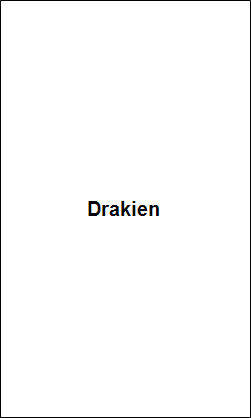
\includegraphics[height=409pt,keepaspectratio]{resources/Drakien.png}
\end{multicols}
\newpage
\begin{multicols}{2}
\subsection{Dune Lizards}
“Friends are not plentiful , to much hatred for us since the Devourer Wars” - Amagat Barakis - Mage of Gallamor
The Lizards are warm blooded and they were once as numerous as the Human race but they made an error of picking the wrong side during the Devourer Wars that resulted in the other races committing mass genocide upon their race. Only the Dune Lizards remain and since the Cataclysm they are not hated as they once were but some of the races with longer lifespans tend to view them with distrust. They are Proud and Loyal and this tendency has sometimes led to their undoing.
Appearance 
Dune Lizards are tall, humanoid reptilian beings shaped by the harsh environments of the desert. Their physiques are built for endurance and survival, with dense musculature, thick hide-like scales, and an imposing presence.
Their skin is made of rough, scaled plates in desert-adapted tones—ranging from sun-bleached sand and muted grey to earthen rust and deep slate. Bone protrusions are commonly visible on the head, forehead, or jawline, giving many individuals a naturally armoured look. Their heads are distinctly lizard-like: elongated, with slitted nostrils, sharp eyes, and no visible external ears. Their eyes are typically reptilian—bright, reflective, and well-suited for navigating both searing daylight and moonlit dunes.
Each hand and foot ends in four digits tipped with curved talons, capable of gripping, climbing, and slashing. Their tails, though often partially hidden beneath layered desert wrappings or armour, provide balance and can be used in combat or defence.
Height and Weights
Dune Lizards Male and Female height is very similar between 5'5ft - 6'5ft. Dune Lizard females are slightly broader than males but average weight is 85-140kg.
Life Expectancy
Their lifetime commonly ranges from 70-90 years due to their constitution. Has a normal sleeping pattern like humans.
Attributes Maximum
\begin{itemize}
\item Strength: 6
\item Agility: 6
\item Constitution: 8
\item Intelligence: 6
\item Wisdom: 6
\item Perception: 6
\item Magic/Faith: 6
\end{itemize}
Attribute Points: 4
Racial Attributes: Constitution +2
Attributes Average
Dune Lizards will often have an Average of 3 in each individual attribute except Constitution where it is normally 5, however these can increase by an additional 1 point in a given profession.
Favoured Profession
Dune Lizards can suit a variety of Roles and are not known to stick to one single profession.
Racial Perks
\MakePerkLink{Night Vision}, \MakePerkLink{Enhanced Smell}, \MakePerkLink{Leathery Skin}.
\begin{itemize}
\item Perk Points: 35
\item Legacy Points: 3
\item Base Movement: 4
\end{itemize}
Gods Worshipped: All
\end{multicols}
\newpage
%%-------------------------------------------------------------------------
% Include this at the start of a Chapter Same level as _Main.tex You should then
% be able to make it as a stand alone text file.
% Make sure you add the footer too!!!
\providecommand{\inmain}{0} % if undefined, assume standalone

\ifnum\inmain=0
  \documentclass[12pt]{article}
  \usepackage[a4paper, margin=1.5cm]{geometry}
  
\usepackage{customPackages/mylinks}
\usepackage{customPackages/loh_skills}
\usepackage{customPackages/loh_perks}

\usepackage{hyperref} % For links and references
\usepackage{makeidx}  % for the Indexing.

\usepackage{longtable}      % for the table itself
\usepackage{array}          % for \newcolumntype (centered text in table)

\usepackage{xparse}     % Optional Argument Stuff IfNoValueTF

\usepackage{graphicx}
\usepackage{multicol}
\usepackage{ragged2e}
\usepackage{lipsum}
\usepackage{fancyhdr}
\usepackage{makeidx}
\usepackage{hyperref}
\usepackage{parskip}
\usepackage{titlesec}
\usepackage{tikz}
\usepackage{eso-pic}
\usepackage{xcolor}
\usepackage{tabularx}
\usepackage{tabularray}
\UseTblrLibrary{booktabs}
\usepackage{longtable}
\usepackage{tocloft}
\usepackage{xcolor}
\usepackage{titlesec}

% used to get the full screen background image stuff to work
\newcommand\SetBackgroundImage[1]{%
  \AddToShipoutPictureBG*{%
    \put(0,0){%
      \parbox[b][\paperheight]{\paperwidth}{%
        \vfill
        \centering
        \includegraphics[width=\paperwidth,height=\paperheight]{#1}%
        \vfill
      }%
    }%
  }%
}

% used to get the full screen background image stuff to work
\newcommand\ClearBackgroundImage{%
  \ClearShipoutPictureBG
}

% Define a custom command for subsubsubsection
% these are NOT sections, but should allow us to play with headings and suchlike.
\usepackage{xcolor} % optional, for color
\newcommand{\subsubsubsection}[1]{%
  \vspace{1em} % vertical space before
  \noindent\textbf{\small #1}\par
  \vspace{0.5em} % vertical space after
}

\input{include/formatting_TOC.tex}

\makeindex
\pagestyle{fancy}
\fancyhf{}
\lhead{POC Document}
\rhead{\thepage}

  \begin{document}
\fi
\subsection{Birthplaces}
This section is about establishing the origin of your character, where they were born and the environment they grew up in. The birthplace you select will influence your character's skills, perks, and potentially their story. Keep in mind that your character's race must match one of the options in the province or country, or you will need to provide an in-game explanation for why your character originates there.
Picking Birthplace
Choose Continent of Birth and gain the Language of that Continent and the Bonus.
Choose the Area that you were born in that's below the continent that you selected and gain the associated language or Skill Ranks, however bear in mind that some areas may not be applicable if your race is not local to the area.
\subsubsection{Non Jadarag}
If you are not playing in the Jadarag setting the GM can give a different variety of Skills. This can be the following:
\begin{itemize}
\item A Language at Skill Rank 6
\item A Racial/Kingdom specific language at Skill Rank 6 or 2 Skill Points.
\item 8 Skill Points: 2 Points for Combat Skill, 1 Point For Non-Combat Skill however if a Read or Write Skill you gain 2 Ranks for the price of 1.
\end{itemize}
\subsubsection{Jadarag}
\subsubsection{Isles of Appia}
\subsubsubsection{Duchy of Calradia}
\subsubsubsection{Kingdom of Andrastes}
\subsubsection{Continent of Ardonia}
Ardonia is a vast and culturally diverse continental realm forged from the remnants of ancient empires, divine wars, and shattered alliances. It spans across fertile plains, jagged mountain ranges, highland forests, and war-torn borders, and is home to a web of interconnected governments, each rooted in shared history but divided by geography, ideology, and ambition.
Ardonia is governed by noble houses who operate within semi-autonomous realms, tied together by shared faiths, trade routes, and historical treaties. The people of Ardonia are very professional and proud of their jobs.
\begin{itemize}
\item Language Common 6
\item 4 Professional Skill Points.
\item 1 Professional Skill may start at Rank 7.
\item \MakePerkLink{Minor Contact} in a different Kingdom.
\end{itemize}
\input{Backgrounds/Birthplaces/Ardonia/Alliance of Daetarre}
\input{Backgrounds/Birthplaces/Ardonia/Breakland of Daetarre} \newpage
\subsection{Stages of development}
\subsubsection{Bloodline}
\subsubsection{Upbringing}
\subsubsection{Adolescence}
\subsubsection{Heritage}
\subsubsection{Development Table}
\subsection{Stages of development}
\subsubsection{Arcane Education}
\subsubsection{Bastion of Arms}
\ifnum\inmain=0
  \end{document}
\fi % See Header		\newpage
% Include this at the start of a Chapter Same level as _Main.tex You should then
% be able to make it as a stand alone text file.
% Make sure you add the footer too!!!
\providecommand{\inmain}{0} % if undefined, assume standalone

\ifnum\inmain=0
  \documentclass[12pt]{article}
  \usepackage[a4paper, margin=1.5cm]{geometry}
  
\usepackage{customPackages/mylinks}
\usepackage{customPackages/loh_skills}
\usepackage{customPackages/loh_perks}

\usepackage{hyperref} % For links and references
\usepackage{makeidx}  % for the Indexing.

\usepackage{longtable}      % for the table itself
\usepackage{array}          % for \newcolumntype (centered text in table)

\usepackage{xparse}     % Optional Argument Stuff IfNoValueTF

\usepackage{graphicx}
\usepackage{multicol}
\usepackage{ragged2e}
\usepackage{lipsum}
\usepackage{fancyhdr}
\usepackage{makeidx}
\usepackage{hyperref}
\usepackage{parskip}
\usepackage{titlesec}
\usepackage{tikz}
\usepackage{eso-pic}
\usepackage{xcolor}
\usepackage{tabularx}
\usepackage{tabularray}
\UseTblrLibrary{booktabs}
\usepackage{longtable}
\usepackage{tocloft}
\usepackage{xcolor}
\usepackage{titlesec}

% used to get the full screen background image stuff to work
\newcommand\SetBackgroundImage[1]{%
  \AddToShipoutPictureBG*{%
    \put(0,0){%
      \parbox[b][\paperheight]{\paperwidth}{%
        \vfill
        \centering
        \includegraphics[width=\paperwidth,height=\paperheight]{#1}%
        \vfill
      }%
    }%
  }%
}

% used to get the full screen background image stuff to work
\newcommand\ClearBackgroundImage{%
  \ClearShipoutPictureBG
}

% Define a custom command for subsubsubsection
% these are NOT sections, but should allow us to play with headings and suchlike.
\usepackage{xcolor} % optional, for color
\newcommand{\subsubsubsection}[1]{%
  \vspace{1em} % vertical space before
  \noindent\textbf{\small #1}\par
  \vspace{0.5em} % vertical space after
}

\input{include/formatting_TOC.tex}

\makeindex
\pagestyle{fancy}
\fancyhf{}
\lhead{POC Document}
\rhead{\thepage}

  \begin{document}
\fi
\section{Professions}
\subsection{Bounty Hunter}
\subsection{Hunter}
\subsection{Journeyman Craftsman}
\ifnum\inmain=0
  \end{document}
\fi % See Header		\newpage
% Include this at the start of a Chapter Same level as _Main.tex You should then
% be able to make it as a stand alone text file.
% Make sure you add the footer too!!!
\providecommand{\inmain}{0} % if undefined, assume standalone

\ifnum\inmain=0
  \documentclass[12pt]{article}
  \usepackage[a4paper, margin=1.5cm]{geometry}
  
\usepackage{customPackages/mylinks}
\usepackage{customPackages/loh_skills}
\usepackage{customPackages/loh_perks}

\usepackage{hyperref} % For links and references
\usepackage{makeidx}  % for the Indexing.

\usepackage{longtable}      % for the table itself
\usepackage{array}          % for \newcolumntype (centered text in table)

\usepackage{xparse}     % Optional Argument Stuff IfNoValueTF

\usepackage{graphicx}
\usepackage{multicol}
\usepackage{ragged2e}
\usepackage{lipsum}
\usepackage{fancyhdr}
\usepackage{makeidx}
\usepackage{hyperref}
\usepackage{parskip}
\usepackage{titlesec}
\usepackage{tikz}
\usepackage{eso-pic}
\usepackage{xcolor}
\usepackage{tabularx}
\usepackage{tabularray}
\UseTblrLibrary{booktabs}
\usepackage{longtable}
\usepackage{tocloft}
\usepackage{xcolor}
\usepackage{titlesec}

% used to get the full screen background image stuff to work
\newcommand\SetBackgroundImage[1]{%
  \AddToShipoutPictureBG*{%
    \put(0,0){%
      \parbox[b][\paperheight]{\paperwidth}{%
        \vfill
        \centering
        \includegraphics[width=\paperwidth,height=\paperheight]{#1}%
        \vfill
      }%
    }%
  }%
}

% used to get the full screen background image stuff to work
\newcommand\ClearBackgroundImage{%
  \ClearShipoutPictureBG
}

% Define a custom command for subsubsubsection
% these are NOT sections, but should allow us to play with headings and suchlike.
\usepackage{xcolor} % optional, for color
\newcommand{\subsubsubsection}[1]{%
  \vspace{1em} % vertical space before
  \noindent\textbf{\small #1}\par
  \vspace{0.5em} % vertical space after
}

\input{include/formatting_TOC.tex}

\makeindex
\pagestyle{fancy}
\fancyhf{}
\lhead{POC Document}
\rhead{\thepage}

  \begin{document}
\fi
\section{Perks and Flaws}
blurb and detials and costs and suchlike go here, don't need the detial on that in the POC
\newpage\subsection{Perks}
\begin{multicols}{2}
\PerkName{Martial Mastery}
\PerkPrereq{\MakeSkillLink{Melee Weapons} 6 (+2 per Level). \MakePerkLink{Toughness}}
\PerkEffect{+1 Damage with \MakeSkillLink{Melee Weapons}}{1}
\PerkEffect{+1 Parry bonus}{2}
\PerkEffect{May make an extra attack once per round.}{3}
\PerkCostPerLevel{5}
%
\PerkName{Night Stalker}
\PerkPrereq{\MakeSkillLink{Stealth} 6, Dexterity 6}
\PerkEffect{Gain +2 to \MakeSkillLink{Stealth} tests made in darkness.}
\PerkCost{4}
%
\PerkName{Sharpshooter}
\PerkPrereq{\MakeSkillLink{Firearms} 8, Perception 7}
\PerkEffect{Ignore -2 penalty for long-range attacks.}
\PerkCost{6}
%
\PerkName{Second Wind}
\PerkPrereq{None}
\PerkEffect{Once per combat, recover 10 percent of max HP as a free action.}
\PerkCost{4}
%
\PerkName{Toughness}
\PerkPrereq{Strength 5}
\PerkEffect{Gain +2 HP}
\PerkCost{3}
%
\PerkName{Weapon Focus (Melee)}
\PerkPrereq{Any Melee Skill at 6}
\PerkEffect{+1 to attack rolls with chosen melee weapon.}
\PerkCost{4}
%
\end{multicols}
\newpage\subsection{Flaws}
\begin{multicols}{2}
\PerkName{Social Outcast}
\PerkEffect{You're awkward, abrasive, or simply uncomfortable around others—whatever the reason, social interaction is not your strength.\\
Whenever you make a social roll involving direct conversation or persuasion (such as Bargain, Con, Persuasion, Leadership, etc.), you must score 1 additional success to achieve a positive outcome.\\
This also applies to opposed social rolls, making it harder to sway or manipulate others in  conversation.}
\PerkCost{1}
\end{multicols}
\ifnum\inmain=0
  \end{document}
\fi % See Header	\newpage
% Include this at the start of a Chapter Same level as _Main.tex You should then
% be able to make it as a stand alone text file.
% Make sure you add the footer too!!!
\providecommand{\inmain}{0} % if undefined, assume standalone

\ifnum\inmain=0
  \documentclass[12pt]{article}
  \usepackage[a4paper, margin=1.5cm]{geometry}
  
\usepackage{customPackages/mylinks}
\usepackage{customPackages/loh_skills}
\usepackage{customPackages/loh_perks}

\usepackage{hyperref} % For links and references
\usepackage{makeidx}  % for the Indexing.

\usepackage{longtable}      % for the table itself
\usepackage{array}          % for \newcolumntype (centered text in table)

\usepackage{xparse}     % Optional Argument Stuff IfNoValueTF

\usepackage{graphicx}
\usepackage{multicol}
\usepackage{ragged2e}
\usepackage{lipsum}
\usepackage{fancyhdr}
\usepackage{makeidx}
\usepackage{hyperref}
\usepackage{parskip}
\usepackage{titlesec}
\usepackage{tikz}
\usepackage{eso-pic}
\usepackage{xcolor}
\usepackage{tabularx}
\usepackage{tabularray}
\UseTblrLibrary{booktabs}
\usepackage{longtable}
\usepackage{tocloft}
\usepackage{xcolor}
\usepackage{titlesec}

% used to get the full screen background image stuff to work
\newcommand\SetBackgroundImage[1]{%
  \AddToShipoutPictureBG*{%
    \put(0,0){%
      \parbox[b][\paperheight]{\paperwidth}{%
        \vfill
        \centering
        \includegraphics[width=\paperwidth,height=\paperheight]{#1}%
        \vfill
      }%
    }%
  }%
}

% used to get the full screen background image stuff to work
\newcommand\ClearBackgroundImage{%
  \ClearShipoutPictureBG
}

% Define a custom command for subsubsubsection
% these are NOT sections, but should allow us to play with headings and suchlike.
\usepackage{xcolor} % optional, for color
\newcommand{\subsubsubsection}[1]{%
  \vspace{1em} % vertical space before
  \noindent\textbf{\small #1}\par
  \vspace{0.5em} % vertical space after
}

\input{include/formatting_TOC.tex}

\makeindex
\pagestyle{fancy}
\fancyhf{}
\lhead{POC Document}
\rhead{\thepage}

  \begin{document}
\fi
\section{Magic and Faith}
\section{Spells and Runes}
\subsection{Defensive}
\subsubsection{Book of Healing}
\subsubsubsection{Salvation}
\subsection{Offensive}
\subsubsection{Book of Air}
\subsubsubsection{Chain Lightning}
\subsubsection{Runes}
\subsubsubsection{Anvil}
\subsubsubsection{Striking}
\ifnum\inmain=0
  \end{document}
\fi % See Header			\newpage
%%-------------------------------------------------------------------------
\section{Equipment}
\section{Combat}
\section{Gods and Religion}











\newpage
\printindex

\end{document}
